% Regarding `oneside` (https://stackoverflow.com/a/8371473/630364):
%
% `oneside` removes the blank pages between chapters.
% "Note that this method make the margins of all the pages the same. In
% `twoside`, the margins are different for the odd and the even pages".
\documentclass[12pt, letterpaper, oneside]{book}

\usepackage{amsfonts}
\usepackage{amsmath}
\usepackage{amssymb}
\usepackage{csquotes}
\usepackage{float}
\usepackage[letterpaper, textwidth=7.5in, textheight=8in]{geometry}
\usepackage{hyperref}
\usepackage{parskip}
\usepackage{pseudocode}
\usepackage{tikz}
\usetikzlibrary{arrows, automata, positioning, shapes.geometric}
\usepackage{titlesec}
\usepackage{xcolor}

\hypersetup{
  colorlinks=true,
  linkcolor=blue,
  filecolor=magenta,
  urlcolor=blue,
}

\setcounter{secnumdepth}{4}

\title{
  Notes on \textit{Stanford: CS103: Mathematical Foundations of Computing}
}
\author{Yaobin Wen}
\date{July 2023}

\begin{document}

\maketitle
\tableofcontents

\chapter*{Overview}
\addcontentsline{toc}{chapter}{Overview}

This document contains my study notes of the Stanford course \textit{CS103:
  Mathematical Foundations of Computing}. I use it for a few purposes:

\begin{enumerate}
  \item As a reference to quickly refresh my memory on the subjects.
  \item Keep the notes to help me understand the text that is not obvious for
        me to comprehend.
\end{enumerate}

% =============================================================================
%
% Set Theory
%
% =============================================================================

\chapter{Set Theory}

% =============================================================================
\section{Is 0 a natural number?}
% =============================================================================

Is $0$ a natural number? Does $\mathbb{N}$ include $0$?

There is no ``yes'' or ``no'' answer to these questions. Take a look at
\href{https://math.stackexchange.com/q/283/665777}{this question} and you will
find people all over the world have all kinds of understanding such as:
\begin{itemize}
  \item $0$ is definitely \textbf{NOT} a natural number and does not belong to
        $\mathbb{N}$.
  \item There are two conventions: In one convention, $0$ is not a natural
        number; in another convention, $0$ is a natural number.
  \item Natural numbers include 0; those positive integers are called ``whole
        numbers'':
        \begin{displayquote}
          I see plenty of both these days, but when I was at school and at
          university, I almost only saw them defined to be {0, 1, ..}. The elements
          of {1, 2, ..} were called the whole numbers in my school days.
        \end{displayquote}
  \item Natural numbers don't include 0; whole numbers, denoted as $\mathbb{W}$,
        include $0$.
  \item $\mathbb{N}$ includes 0; $\mathbb{N^+}$ is all the positive integers so
        it doesn't include 0.
  \item yadda yadda yadda...
\end{itemize}

So I don't think it makes sense to argue whether $0$ is a natural number or not.
We just need to define it clearly and move on.

In CS103, $\mathbb{N}$ represents the natural numbers that \textbf{include} $0$.
But if you read 18.100A, you'll see in that course, $\mathbb{N}$ does not
include $0$.

That's fine. The world is still in peace. So in this note, I will respect the
choice of CS103 and treat $\mathbb{N}$ as the set of all the non-negative
integers, i.e., \[\{0, 1, 2, 3, \ldots\}\].

% =============================================================================
\section{Introduction to Set Theory}
% =============================================================================

This first lecture introduces set theory. Because I have learned them in MIT
OCW 18.100A Real Analysis, I won't repeat the notes again because they can be
found in the notes for that course. Here, I will just mention a few points that
are not covered in 18.100A.

\begin{itemize}
  \item Set difference: 18.100A uses $A \setminus B$ to denote ``A minus B''.
        CS103 says $A - B$ is also used.
  \item \textbf{Symmetric difference}: $A \bigtriangleup B = (A \setminus B)
          \cup (B \setminus A) = (A \cup B) \setminus (A \cap B)$. For example, if
        $A = \{1, 2, 3\}$ and $B = \{3, 4, 5\}$, then $A \bigtriangleup B = \{1, 2,
          4, 5\}$. \colorbox{red}{\textcolor{yellow}{TODO:}} Add a Venn diagram.
\end{itemize}

% =============================================================================
\section{Cardinality}
% =============================================================================

% ******************************
\subsection{$|\mathbb{N}|$ and $|\mathbb{Z}|$}
% ******************************

I've already learned that $|\mathbb{Z}|$ and the set of all the even (or odd)
numbers have the same cardinality, but in CS103 I just learned $|\mathbb{N}| =
  |\mathbb{Z}|$. The bijection (see 18.100A) between $\mathbb{N}$ and $\mathbb{Z}$
is created in the following way:
\begin{itemize}
  \item All the non-negative even numbers (including $0$) in $\mathbb{N}$ are
        matched to one non-negative integers in $\mathbb{Z}$.
  \item All the non-negative odd numbers in $\mathbb{N}$ are matched to one
        negative integers in $\mathbb{Z}$.
\end{itemize}

Visualized, this can be shown as:
\begin{itemize}
  \item $0 \longleftrightarrow 0$
  \item $1 \longleftrightarrow -1$
  \item $2 \longleftrightarrow 1$
  \item $3 \longleftrightarrow -2$
  \item $4 \longleftrightarrow 2$
  \item $5 \longleftrightarrow -3$
  \item $6 \longleftrightarrow 3$
  \item $7 \longleftrightarrow -4$
  \item $8 \longleftrightarrow 4$
  \item etc.
\end{itemize}

In general, the bijection $f: \mathbb{N} \rightarrow \mathbb{Z}$ is defined as:

\[
  f(n) = \begin{cases}
    n / 2,        & if \ MOD(n) = 0 \\
    (-n - 1) / 2, & if \ MOD(n) = 1
  \end{cases}
\]

where $n \in \mathbb{N}$.

% ******************************
\subsection{Cantor's diagonalization proof}
% ******************************

\href{https://en.wikipedia.org/wiki/Cantor%27s_diagonal_argument}{Cantor's
  diagonalization proof} is used to prove $|S| < |\mathcal{P}(S)|$.

% ******************************
\subsection{$|Programs| < |Problems|$}
% ******************************

This is the most interesting conclusion I've seen in this lecture. The proof
process can be summarized as follows:
\begin{itemize}
  \item Because every valid computer program is essentially a string, but not
        every string is a valid program, we can see \[|Program| \leq |Strings|\].
  \item The problems in the world may or may not deal with sets of strings.
        Suppose $S$ denotes a set of strings, so one kind of problems is: Given a
        string $s$, determine whether $s \in S$. For example:
        \begin{itemize}
          \item Suppose S = \{ ``a'', ``b'', ``c'', $\ldots$, ``z'' \}, then the
                problem can be: Given a string $s$, determine whether $s$ is an English
                letter.
          \item Suppose S = \{ ``0'', ``1'', ``2'', ``3'', $\ldots$ \}, then the
                problem can be: Given a string $s$, determine whether $s$ represents a
                natural number.
        \end{itemize}
  \item Not to mention that other kinds of problems can exist and may not be
        converted to problems that deal with sets of strings.
  \item The conclusion is: $|Sets\ of\ strings| \leq |Problems|$. They could be
        equal, if all the problems can be converted to problems that deal with sets
        of strings.
  \item Therefore:
        \[|Program| \leq |Strings| < |Sets\ of\ strings| \leq |Problems|\]
\end{itemize}

% =============================================================================
%
% Mathematical Proofs
%
% =============================================================================

\chapter{Mathematical Proofs}

\begin{enumerate}
  \item $\blacksquare$ means ``end of proof''.
  \item Use the ``mugga mugga'' test to verify if the proof is written in valid
        sentences: Replace all the mathematical notation with ``mugga mugga''. What
        comes back should still be a valid sentence.
  \item The section ``Proofs as a Dialog'' is interesting: It says the variables
        used in a proof can be divided into three categories:
        \begin{enumerate}
          \item Proof writer picks. Example: ``Let r = n + 1''
          \item Proof reader picks. Example: ``Consider some $n \in \mathbb{N}$''
          \item Neither picks: The variable's value is determined by some laws or
                definition. Example: ``If $n$ is even, there exists a $k$ so that $n =
                  2k$''. In this case, if the reader chooses an arbitrary even number $n$,
                the corresponding $k$'s value is not chosen by either the reader or the
                writer but by the definition of ``even''.
        \end{enumerate}
        Knowing which variables are picked by whom can help verify if the proof
        makes sense. Don't change the variables you (the proof writer) don't own.
\end{enumerate}

% =============================================================================
%
% Indirect Proofs
%
% =============================================================================

\chapter{Indirect Proofs}

% =============================================================================
\section{Implication}
% =============================================================================

An implication can be denoted as $p \rightarrow q$:
\begin{enumerate}
  \item In mathematics, implication is directional.
  \item In mathematics, implications only say something about the consequent
        when the antecedent is true.
  \item In mathematics, implication says nothing about causality.
\end{enumerate}

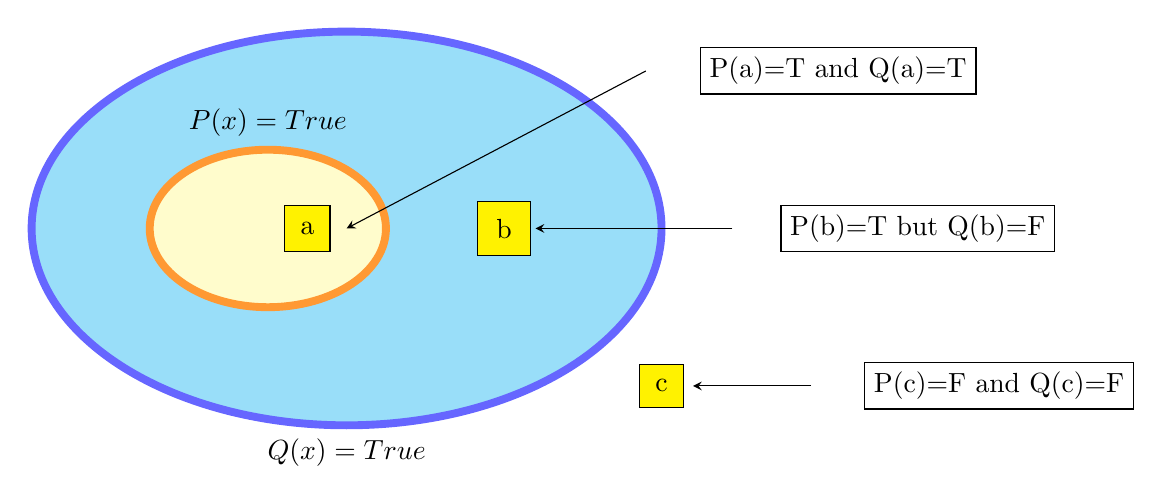
\begin{tikzpicture}
  % Set Q, the enclosing set.
  \node [ellipse,
    draw=blue!60,
    fill=cyan!40,
    line width=1mm,
    minimum width=8cm,
    minimum height=5cm,
    label={-90:$Q(x)=True$}] (Q) at (0,0) {};

  % Set P, the enclosed set.
  \node [ellipse,
    draw=orange!80,
    fill=yellow!20,
    line width=1mm,
    minimum width=3cm,
    minimum height=2cm,
    label={$P(x)=True$}] (P) at (-1,0) {};

  % Element a where P(a) = True and Q(a) = True
  \node [
    regular polygon,
    draw,
    regular polygon sides=4,
    minimum size=0.5cm,
    fill=yellow] (a) at (-0.5,0) {a};
  \node[
    draw=black,
    left, black, fill=white] at (8,2) {P(a)=T and Q(a)=T};
  \draw [-stealth] (3.8,2) -- (0,0);

  % Element b where P(b) = True but Q(b) = False
  \node [
    regular polygon,
    draw,
    regular polygon sides=4,
    minimum size=0.5cm,
    fill=yellow] (b) at (2,0) {b};
  \node[
    draw=black,
    left, black, fill=white] at (9,0) {P(b)=T but Q(b)=F};
  \draw [-stealth] (4.9,0) -- (2.4,0);

  % Element c where P(c) = True and Q(c) = True
  \node [
    regular polygon,
    draw,
    regular polygon sides=4,
    minimum size=0.5cm,
    fill=yellow] (c) at (4,-2) {c};
  \node[
    draw=black,
    left, black, fill=white] at (10,-2) {P(c)=F and Q(c)=F};
  \draw [-stealth] (5.9,-2) -- (4.4,-2);
\end{tikzpicture}

% =============================================================================
\section{Negation}
% =============================================================================

The negation of the \textbf{universal} statement is the \textbf{existential}
statement:
\begin{enumerate}
  \item ``Every P is a Q'' $\rightarrow$ ``There is a P that is not a Q''
  \item ``$\forall x: P(x)=True$'' $\rightarrow$ ``$\exists x: P(x)=False$''
\end{enumerate}

The negation of the \textbf{existential} statement is the \textbf{universal}
statement:
\begin{enumerate}
  \item ``There exists a P that is a Q'' $\rightarrow$ ``Every P is not a Q''
  \item ``$\exists x: P(x)=True$'' $\rightarrow$ ``$\forall x: P(x)=False$''
\end{enumerate}

% -----------------------------------------------------------------------------
\subsection{Negate an implication}
% -----------------------------------------------------------------------------

How to negate the implication:

\begin{displayquote}
  If Nanni pays money to Ea-Nasir, then Ea-Nasir will give Nanni quality copper
  ingots.
\end{displayquote}

An implication should be viewed as in the form as follows:

\begin{displayquote}
  For any x, if P(x) is true, then Q(x) is also true.
\end{displayquote}

Therefore the implication above should be re-interpretted as follows:

\begin{displayquote}
  For any time when Nanni pays money to Ea-Nasir, then Ea-Nasir will give Nanni
  quality copper ingots.
\end{displayquote}

So the negation of the concerned implication is:

\begin{displayquote}
  There are times when Nanni pays money to Ea-Nasir, then Ea-Nasir does not
  give Nanni quality copper ingots.
\end{displayquote}

% =============================================================================
\section{Proof by Contrapositive}
% =============================================================================

The contrapositive of the implication

\begin{displayquote}
  If \textbf{\textcolor{teal}{P is true}}, then \textbf{\textcolor{violet}{Q is
      true}}
\end{displayquote}

is the implication

\begin{displayquote}
  If \textbf{\textcolor{violet}{Q is false}}, then \textbf{\textcolor{teal}{P
      is false}}.
\end{displayquote}

They are \textbf{equivalent}.

To prove the original proposition, one can prove its contrapositive, hence
``proof by contrapositive''.

% =============================================================================
\section{Biconditionals}
% =============================================================================

Biconditionals are the ``if and only if''s, namely $p \Leftrightarrow q$.

To prove a biconditional, we must prove two directions: $p \Rightarrow q$ and
$q \Rightarrow p$.

% =============================================================================
\section{Proof by contradiction}
% =============================================================================

Example of how to write a proof by contradiction:

\begin{displayquote}
  Theorem: There is no largest set.

  Proof: \textbf{\textcolor{violet}{Assume for the sake of contradiction}} that
  \textbf{\textcolor{orange}{there is a largest set; call it $S$}}.

  (Steps to show the contradiction.)

  (Conclusion) \textbf{\textcolor{teal}{We've reached a contradiction, so our
      assumption must have been wrong. Therefore, there is no largest set.}}
  $\blacksquare$
\end{displayquote}

% =============================================================================
%
% Propositional Logic
%
% =============================================================================

\chapter{Propositional Logic}

% =============================================================================
\section{Proposition}
% =============================================================================

% ******************************
\subsection{Definition}
% ******************************

A \textbf{proposition} is a statement that is, by itself, either \textbf{true}
or \textbf{false}.
\begin{itemize}
  \item Commands are not propositions. Example: Open the door.
  \item Questions are not propositions. Example: What day is it today?
\end{itemize}

A \textbf{propositional variable}, usually a lower-case English letter such as
$p$, $q$, $r$, represents a proposition.

A \textbf{propositional connective} expresses how propositions are related.
Some of the connectives are:
\begin{itemize}
  \item $\lnot p$: ``NOT p''; logical negation.
  \item $p \land q$: ``p AND q''; logical conjunction.
  \item $p \lor q$: ``p OR q''; logical disjunction (inclusive). ``inclusive''
        means $p$ and $q$ can be $true$ at the same time, while ``exclusive or''
        means $p$ and $q$ cannot be $true$ at the same time.
  \item $p \rightarrow q$: ``p implies q''; material condition.
  \item $p \leftrightarrow q$: ``p if and only if q'', which also means ``(p
        implies q) AND (q implies p)''.
  \item $\top$: ``(always) true'' ($\top$ looks like a upper-case ``T'' that
        can represent ``True''.)
  \item $\bot$: ``(always) false''
\end{itemize}

% ******************************
\subsection{Example of using $\top$ and $\bot$}
% ******************************

$\bot$ can be used to describe how proof by contradiction works. Suppose that
you want to prove $p$ is $true$ using proof by contradiction. The usual steps
are as follows:
\begin{enumerate}
  \item Assume $p$ is $false$.
  \item Derive a conclusion that is known as $false$ (e.g., ``3 is even'').
  \item Conclude that $p$ is $true$.
\end{enumerate}

Described in propositional logic, it is
\[
  (\lnot p \rightarrow \bot) \rightarrow p
\].

% ******************************
\subsection{Logical operator precedence}\label{logical_operator_precedence}
% ******************************

All the logical operators are \textbf{right-associative}.

In the order of highest to lowest, they are:
\begin{enumerate}
  \item $\lnot$
  \item $\land$
  \item $\lor$
  \item $\rightarrow$
  \item $\leftrightarrow$
\end{enumerate}

For example, the statement
\[
  \lnot x \rightarrow y \lor z \rightarrow x \lor y \and z
\]
can be grouped as follows:
\[
  (\lnot x) \rightarrow ((y \lor z) \rightarrow (x \lor (y \and z)))
\]

% ******************************
\subsection{Truth table}
% ******************************

I have already learned the truth tables for $\lnot$, $\land$, and $\lor$. What
is surprising to me is the truth table for $\rightarrow$:

\begin{table}[H]
  \centering
  \begin{tabular}{|c|c|c|ll}
    \cline{1-3}
    p & q & $p \rightarrow q$ &  & \\ [1ex] \cline{1-3}
    F & F & T                 &  & \\ [0.5ex] \cline{1-3}
    F & T & T                 &  & \\ [0.5ex] \cline{1-3}
    T & F & F                 &  & \\ [0.5ex] \cline{1-3}
    T & T & T                 &  & \\ [0.5ex] \cline{1-3}
  \end{tabular}
  \caption{Truth table for $p \rightarrow q$}
\end{table}

The first two lines are the most confusing to many people, and there are many
questions about them. Here are some of them:
\begin{itemize}
  \item \href{https://philosophy.stackexchange.com/q/26719/44172}{Shouldn't statements be considered equivalent based on their meaning rather than truth tables?}
  \item \href{https://philosophy.stackexchange.com/q/34082/44172}{Why are conditionals with false antecedents considered true?}
  \item \href{https://math.stackexchange.com/q/3098664/665777}{How Implication or Material/Concrete Conditional works when the antecedent is false and the consequent is true}
  \item \href{https://math.stackexchange.com/q/70736/665777}{In classical logic, why is ($p \rightarrow q$) True if p is False and q is True?}
  \item And many more...
\end{itemize}

I read some of the posts and then decided to stop because this looks like a
deep rabbit hole. For now, it is better to just accept the truth table and move
on. But to help understand them a little bit:
\begin{itemize}
  \item $p \rightarrow q \equiv \lnot p \lor q \equiv \lnot (p \land \lnot q)$.
  \item $\lnot (p \rightarrow q) \equiv p \land \lnot q$.
  \item It's helpful to think about ``Ex falso sequitur quodlibet'' which means
        ``from what is false any assertion validly follows''.
\end{itemize}

\colorbox{red}{\textcolor{yellow}{TODO:}} Figure out why $F \rightarrow F$ is
$T$ and $F \rightarrow T$ is $T$. Or figure out why $p \rightarrow q$ is
equivalent to $\lnot p \lor q$.

Here is the truth table for $p \leftrightarrow q$:

\begin{table}[H]
  \centering
  \begin{tabular}{|c|c|c|ll}
    \cline{1-3}
    p & q & $p \leftrightarrow q$ &  & \\ [1ex] \cline{1-3}
    F & F & T                     &  & \\ [0.5ex] \cline{1-3}
    F & T & F                     &  & \\ [0.5ex] \cline{1-3}
    T & F & F                     &  & \\ [0.5ex] \cline{1-3}
    T & T & T                     &  & \\ [0.5ex] \cline{1-3}
  \end{tabular}
  \caption{Truth table for $p \rightarrow q$}
\end{table}

% ------------------------------
\subsubsection{Vacuously true; trivially true}
% ------------------------------

An implication with a false antecedent is called \textbf{vacuously true}, such
as $F \rightarrow F: T$ and $F \rightarrow T: T$.

An implication with a true consequent is called \textbf{trivially true}, such
as $F \rightarrow T: T$ and $T \rightarrow T: T$.

Note that the implication $F \rightarrow F: T$ is \textbf{both vacuous and
  trivial}.

Note that the implication $T \rightarrow F: F$ is \textbf{neither of them}.

% ******************************
\subsection{de Morgan's Laws}
% ******************************

\begin{itemize}
  \item $\lnot (p \land q) \equiv \lnot p \lor \lnot q$
  \item $\lnot (p \lor q) \equiv \lnot p \land \lnot q$
\end{itemize}

% =============================================================================
%
% First-Order Logic
%
% =============================================================================

\chapter{First-Order Logic}

% =============================================================================
\section{What is First-Order Logic?}
% =============================================================================

First-order logic:
\begin{enumerate}
  \item It is a a logical system for reasoning about properties of objects.
        There are two kinds of objects:
        \begin{enumerate}
          \item \textbf{Constants}: A symbol that refers to a specific object. For
                example, ``You'', ``Me'', ``EastAtlanta'', ``137''. Note that
                numbers such as ``137'' are \textbf{not} built in to first-order logic.
                They are just constant symbols like ``You'' and ``Me''.
          \item \textbf{Variables}: A symbol that serves as a placeholder to
                represent any object in a particular set. Usually this is used when
                \textbf{quantifiers} is used (because when quantifiers are used, we
                don't specify just one specific object, so we need a symbol to
                represent any of such objects we are referring to).
        \end{enumerate}
  \item It is built upon propositional logic.
  \item It uses the following three devices to describe more complex logic:
        \begin{enumerate}
          \item \textbf{predicates}: Describe \textbf{properties} of objects. It
                can take one or more objects as input and turn them into a proposition
                which is evaluated as $true$ or $false$.
                \begin{enumerate}
                  \item Binary predicates are sometimes written in \textbf{infix
                          notation}. For example, instead of writing ``$<(x, 8)$'', it's
                        more natural to write ``$x < 8$''.
                \end{enumerate}
          \item \textbf{functions}: Map objects to objects.
          \item \textbf{quantifiers}: Describe the quantities of objects, mainly
                two cases: ``for all objects'' and ``for some objects''.
        \end{enumerate}
  \item Examples:
        \begin{enumerate}
          \item $Likes(You, Eggs) \land Likes(You, Tomato) \rightarrow
                  Likes(You, Shakshuka)$
          \item $In(MyHeart, Havana) \land TookBackTo(Him, Me, EastAtlanta)$
        \end{enumerate}
\end{enumerate}

% =============================================================================
\section{Equality}
% =============================================================================

\begin{enumerate}
  \item The predicates ``$=$'' and ``$\neq$'' indicate whether two
        \textbf{objects} are equal or not.
  \item ``$\leftrightarrow $'' indicates that two \textbf{propositions} are
        equal. Note that ``$\leftrightarrow $'' is not a predicate because
        predicates are applied to objects to describe the objects' properties, but
        ``$\leftrightarrow $'' is applied to propositions to describe their logical
        relations.
\end{enumerate}

% =============================================================================
\section{Type-Checking Table}
% =============================================================================

\begin{table}[H]
  \centering
  \begin{tabular}{|l|l|l|}
    \hline
    \textbf{}            & \textbf{...operate on..} & \textbf{...produce} \\ [1ex] \hline
    \textbf{Connectives} & propositions             & a proposition       \\ [1ex] \hline
    \textbf{Predicates}  & objects                  & a proposition       \\ [1ex] \hline
    \textbf{Functions}   & objects                  & an object           \\ [1ex] \hline
  \end{tabular}
  \caption{Type-Checking Table}
  \label{FOL_type_checking_table}
\end{table}

% =============================================================================
\section{Existential and Universal Quantifiers}
% =============================================================================

% ******************************
\subsection{General form}
% ******************************

The general form of using the quantifiers is as follows:
\begin{enumerate}
  \item $\exists x. PROPERTY(x)$: Some $x$ has the property ``PROPERTY''.
  \item $\forall x. PROPERTY(x)$: All $x$ has the property ``PROPERTY''.
\end{enumerate}

To describe the set that $x$ belongs to, use the following forms:
\begin{enumerate}
  \item $\exists x. (x \in X \rightarrow PROPERTY(x))$
  \item $\forall x. (x \in X \rightarrow PROPERTY(x))$
\end{enumerate}

For example, ``For any natural number $n$, $n$ is even if and only if $n^2$ is
even'' can be translated into
\[
  \forall n. (n \in \mathbb{N} \rightarrow (Even(n) \leftrightarrow Even(n^2)))
\]

% ******************************
\subsection{Edge cases}
% ******************************

I'm familiar with the existential quantifier ``$\exists$'' and the universal
quantifier ``$\forall$'', but I didn't think about the two edge cases before:
\begin{enumerate}
  \item $\exists x. (x \in \emptyset \rightarrow PROPERTY(x) = \bot)$, i.e.,
        existentially-quantified statements are always \textbf{false} in an empty
        world because \textbf{nothing exists}.
  \item $\forall x. (x \in \emptyset \rightarrow PROPERTY(x) = \top)$, i.e.,
        universally-quantified statements are said to be \textbf{vacuously true} in
        an empty world.
\end{enumerate}

% ******************************
\subsection{Association}
% ******************************

The variable is scoped just to the statement being quantified. For example:
\[(\exists x. BIGGER(A, x)) \land (\exists y. SMALLER(y, B))\]

\begin{enumerate}
  \item $x$ is only applicable to ``BIGGER''.
  \item $y$ is only applicable to ``SMALLER''.
\end{enumerate}

% ******************************
\subsection{Precedence}
% ******************************

Quantifiers have precedence just below ``$\lnot$''. See
\ref{logical_operator_precedence}.

Therefore, the statement \[\exists x. P(x) \land R(x) \land Q(x)\] is parsed as
\[(\exists x. P(x)) \land R(x) \land Q(x)\] which is \textbf{syntactically
  invalid} because the variable $x$ is out of scope for $R$ and $Q$.



% =============================================================================
%
% Functions
%
% =============================================================================

\chapter{Functions}

 (TODO)

% =============================================================================
%
% Graphs
%
% =============================================================================

\chapter{Graphs}

 (TODO)

% =============================================================================
%
% Mathematical Induction
%
% =============================================================================

\chapter{Mathematical Induction}

 (TODO)

% =============================================================================
%
% Finite Automata
%
% =============================================================================

\chapter{Finite Automata}

% =============================================================================
\section{Computability Theory}
% =============================================================================

\textbf{Two key questions}: How can we prove what computers can and can't do...
\begin{enumerate}
  \item ... so that our results are still true in 20 years?
  \item ... without multi-hundred page proofs?
\end{enumerate}

% =============================================================================
\section{Finite Automata: Modeling Finite Computation}
% =============================================================================

\colorbox{lime}{\textbf{NOTE(ywen)}}: The automata seem to be different from the ``state machines'' I have understood
so far. The ``state machines'' I've been using are those whose every state is an ``accepting state'' (see below for the
meaning of an ``accepting state''), but an automaton may have accepting states (which the automaton returns ``Yes'' to
indicate the acceptance) and rejecting states (which the automaton returns ``No'' to indicate the rejection). In other
words, the ``state machines'' I've been using all the time are a subset of automata.

Slide 42 says:
\begin{displayquote}
  As a simplifying assumption, we'll assume that we just need to get a single
  bit of output. That is, our machines will just say \textbf{YES} or
  \textbf{NO}.
\end{displayquote}

\colorbox{red}{\textcolor{yellow}{TODO:}} I need to learn how the generalization happens.

Slide 44 introduces the following terms:
\begin{itemize}
  \item \textbf{accepting states}: \colorbox{red}{\textcolor{yellow}{TODO:}}
        How to determine if a state is an accepting state?
  \item \textbf{accepts}: If the device ends in an \textbf{accepting state}
        after seeing all the input, it \textbf{accepts} the input (says
        \textbf{YES}).
  \item \textbf{rejects}: If the device does not end in an \textbf{accepting
          state} after seeing all the input, it \textbf{rejects} the input (says
        \textbf{NO}).
\end{itemize}

Finite automata model computers where:
\begin{enumerate}
  \item memory is finite.
  \item the computation produces as YES/NO answer. (``YES/NO" is similar to
        ``True/False". In other words, given the input, an automaton outputs
        ``True/False", so an automaton can be viewed as a \textbf{predicate}. See
        ``first-order logic'' for the meaning of a ``predicate''.)
\end{enumerate}

% ******************************
\subsection{Finite Automata and Languages}
% ******************************

In order to define finite automata and their languages, we need to define ``languages'' first.

% ------------------------------
\subsubsection{Alphabet}
% ------------------------------

An \textbf{alphabet} is:
\begin{enumerate}
  \item a \textbf{finite}, \textbf{nonempty} set of symbols called \textbf{characters}.
  \item denoted by $\Sigma$.
\end{enumerate}

For example, $\Sigma = \{a, b\}$ is an alphabet over the characters ``a'' and ``b''.

% ------------------------------
\subsubsection{Strings}
% ------------------------------

A \textbf{string} over an alphabet $\Sigma$ is a \textbf{finite} sequence of characters drawn from $\Sigma$. The
\textbf{empty string} has no characters and is denoted $\epsilon$. The set of \textbf{all strings} composed from the
characters in $\Sigma$ is denoted $\Sigma^*$.

For example, some strings over $\Sigma = \{a, b\}$ are: ``a'', ``ababbabbbababba'', ``abbabbab''.

\colorbox{lime}{\textbf{NOTE(ywen)}}: A tip to remember the symbols: In regular expressions in computer science, we use
asterisks (``*'') to denote the quantifier ``repeating the previous item zero or more times''. Therefore, $\Sigma^*$
can be seen as ``repeating the characters in the set of $\Sigma$ zero or more times.'' When it's zero times, the
resulting string is the empty string $\epsilon$; when it's one or more times, the resulting string is a non-empty one.

% ------------------------------
\subsubsection{Languages}
% ------------------------------

A \textbf{language}:
\begin{enumerate}
  \item is a set of \textbf{strings}.
  \item is a language over $\Sigma$ if it is a subset of $\Sigma^*$.
\end{enumerate}

% ------------------------------
\subsubsection{Finite Automata and Languages} \label{automata:automata-and-languages}
% ------------------------------

Let $A$ be an automaton that processes strings drawn from an alphabet $\Sigma$. The language of $A$, denoted
$\mathfrak{L}(A)$, is the set of strings over $\Sigma$ that $A$ accepts:

\[
  \mathfrak{L}(A) = \{ w \in \Sigma^* | A \ accepts \ w \}
\]

Here ``$A$ accepts $w$'' is the general form of the rule about $w$. In a particular example of automaton, it can be
``$w$ ends in the character $a$''.

% ------------------------------
\subsubsection{Summary}
% ------------------------------

\begin{enumerate}
  \item A \textbf{finite automaton} is a collection of \textbf{states} joined by \textbf{transitions}.
  \item Some state is designated as the \textbf{start state}.
  \item Some number of states are designated as \textbf{accepting states}. These accepting states make the automaton
        return ``Yes''.
  \item The automaton processes a string by beginning in the start state and following the indicated transitions.
  \item If the automaton ends in an accepting state, it \textbf{accepts} the input. Otherwise, the automaton
        \textbf{rejects} the input.
  \item The \textbf{language} of an automaton is the set of strings it accepts.
\end{enumerate}

% =============================================================================
\section{Deterministic Finite Automaton (DFA)}
% =============================================================================

% ******************************
\subsection{Two problems of indeterminism}
% ******************************

First problem: \textbf{No transition is defined out of a state on some input.} For example, in the following automaton,
the entire possible input space is $\{0, 1\}$. However, for the states $q_0$ and $q_2$, the transitions on the input
$1$ are \textbf{undefined}; for the state $q_1$, the transition on the input $0$ is \textbf{undefined}.

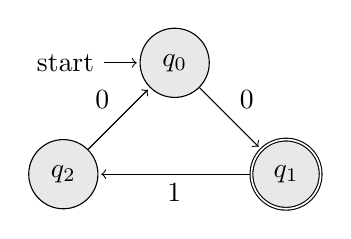
\begin{tikzpicture}[shorten >=1pt,node distance=2cm,auto]
  \tikzstyle{every state}=[fill={rgb:black,1;white,10}]

  \node[state,initial]   (q_0)                      {$q_0$};
  \node[state,accepting] (q_1) [below right of=q_0] {$q_1$};
  \node[state]           (q_2) [below left of=q_0]  {$q_2$};

  \path[->]
  (q_0) edge node {0} (q_1)
  (q_1) edge node {1} (q_2)
  (q_2) edge node {0} (q_0)
  ;
\end{tikzpicture}

Second problem: \textbf{There are multiple transitions out of a state on some input.} For example, in the following
automaton, on the input $0$, the state $q_1$ has two possible out transitions.

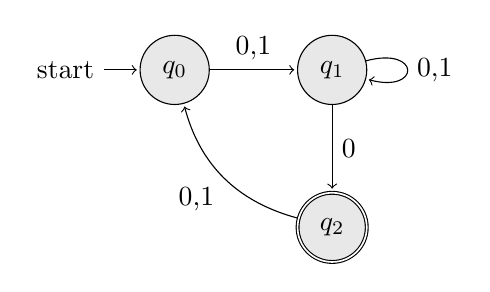
\begin{tikzpicture}[shorten >=1pt,node distance=2cm,auto]
  \tikzstyle{every state}=[fill={rgb:black,1;white,10}]

  \node[state,initial]   (q_0)                 {$q_0$};
  \node[state]           (q_1) [right of=q_0]  {$q_1$};
  \node[state,accepting] (q_2) [below of=q_1]  {$q_2$};

  \path[->]
  (q_0) edge              node {0,1} (q_1)
  (q_1) edge [loop right] node {0,1} (q_1)
  (q_1) edge              node {0}   (q_2)
  (q_2) edge [bend left]  node {0,1} (q_0)
  ;
\end{tikzpicture}

Therefore, in order to reason about the limits of what finite automata can and cannot do, we need to formally specify
their behavior in \textbf{all cases}. All of the following need to be \textbf{defined} or \textbf{disallowed}:
\begin{itemize}
  \item What happens if there is no transition out of a state on some input?
  \item What happens if there are multiple transitions out of a state on some input?
\end{itemize}

% ******************************
\subsection{DFAs}
% ******************************

\begin{itemize}
  \item A DFA is defined relative to some alphabet $\Sigma$.
  \item For each state in the DFA, there must be \textbf{exactly one} transition defined for each symbol in $\Sigma$.
  \item There is \textbf{exactly one} start state.
  \item There are \textbf{zero or more} accepting states.
\end{itemize}

% ------------------------------
\subsubsection{The DFA for valid C-style comments}
% ------------------------------

The problem to solve is to design a DFA that represents any valid C-style comments. We use the symbol ``a'' to be the
placeholder for the characters that are not an asterisk or slash.

Note that the following are valid C-style comments:
\begin{itemize}
  \item /*/*/
  \item /*//*/
  \item /*/***/
\end{itemize}

In my first attempt, I designed the following DFA. Note this design has a few mistakes. See my notes below.

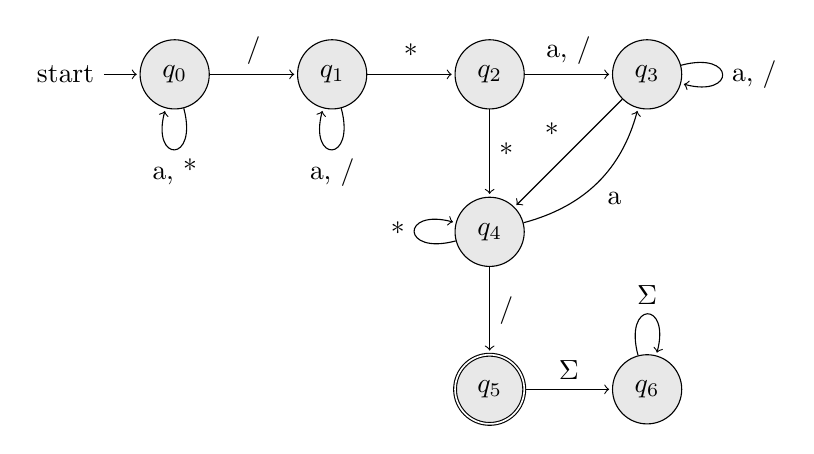
\begin{tikzpicture}[shorten >=1pt,node distance=2cm,auto]
  \tikzstyle{every state}=[fill={rgb:black,1;white,10}]

  \node[state,initial]   (q_0)                 {$q_0$};
  \node[state]           (q_1) [right of=q_0]  {$q_1$};
  \node[state]           (q_2) [right of=q_1]  {$q_2$};
  \node[state]           (q_3) [right of=q_2]  {$q_3$};
  \node[state]           (q_4) [below of=q_2]  {$q_4$};
  \node[state,accepting] (q_5) [below of=q_4]  {$q_5$};
  \node[state]           (q_6) [right of=q_5]  {$q_6$};

  \path[->]
  (q_0) edge                    node {/}        (q_1)
  (q_0) edge [loop below]       node {a, *}     ()
  (q_1) edge                    node {*}        (q_2)
  (q_1) edge [loop below]       node {a, /}     ()
  (q_2) edge                    node {a, /}     (q_3)
  (q_2) edge                    node {*}        (q_4)
  (q_3) edge [loop right]       node {a, /}     ()
  (q_3) edge [swap]             node {*}        (q_4)
  (q_4) edge [bend right, swap] node {a}        (q_3)
  (q_4) edge [loop left]        node {*}        ()
  (q_4) edge                    node {/}        (q_5)
  (q_5) edge                    node {$\Sigma$} (q_6)
  (q_6) edge [loop above]       node {$\Sigma$} ()
  ;
\end{tikzpicture}

Unfortunately, there are a few errors in this design:
\begin{enumerate}
  \item On the state $q_0$, the edge \{a, *\} that goes into itself is wrong because it means if a ``/'' follows a
        bunch of ``a'' and ``*'', the result can still be a valid C-style comment. For example, ``a/a/aa/*aa*/'' is
        not a valid C-style comment, but my DFA would consider it valid, which is an error. \textbf{The lesson:} When
        validating the design, we need to use three \textbf{types} of input:
        \begin{enumerate}
          \item \textbf{Full valid} input. For example, ``/* aaa */'' is a full valid input.
          \item \textbf{Full invalid} input. For example, ``*//**'' is a full invalid input.
          \item \textbf{Partial invalid (valid prefix + invalid suffix)} input. For example, ``/* a */*/**''. The
                former part ``/* a */'' is a valid input but the latter part ``*/**'' is an invalid input.
          \item \textbf{Partial invalid (invalid prefix + valid suffix)} input. For example, ``*/**/* a */''. The
                former part ``*/**'' is an invalid input but the latter part ``/* a */'' is a valid input.
        \end{enumerate}
  \item Likewise, on the state $q_1$, the edge \{a, /\} that goes into itself is wrong for the similar reason. For
        example, ``/a/aaa*a*/'' is not a valid C-style comment, but my DFA would consider it valid.
  \item The states $q_2$ and $q_3$ are equivalent and can be merged as one state. One way to check if two states are
        \textbf{possibly} redundant can be checking whether the two states have the same out-transitions. In my DFA,
        the state $q_2$ has two out-transitions: the edge \{a, /\} to $q_3$ and the edge \{*\} to $q_4$. The state
        $q_3$ has the same two out-transitions. This means $q_2$ and $q_3$ may be equivalent and should be examined
        more closely.
\end{enumerate}

The correct DFA should be the following one (which is equivalent to the one in the course slides):

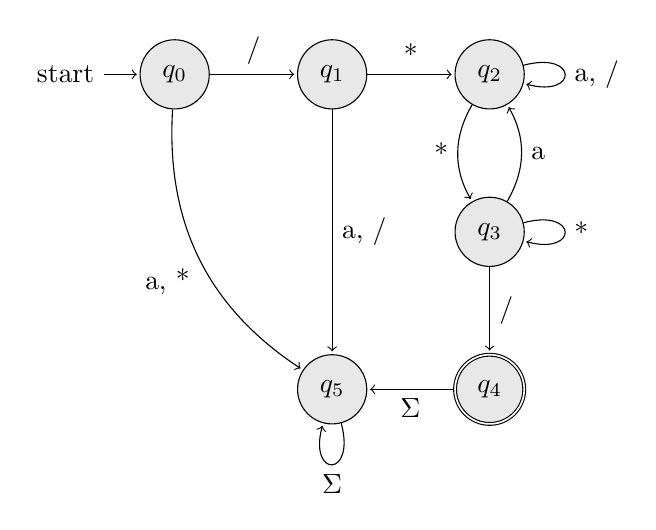
\begin{tikzpicture}[shorten >=1pt,node distance=2cm,auto]
  \tikzstyle{every state}=[fill={rgb:black,1;white,10}]

  \node[state,initial]   (q_0)                 {$q_0$};
  \node[state]           (q_1) [right of=q_0]  {$q_1$};
  \node[state]           (q_2) [right of=q_1]  {$q_2$};
  \node[state]           (q_3) [below of=q_2]  {$q_3$};
  \node[state,accepting] (q_4) [below of=q_3]  {$q_4$};
  \node[state]           (q_5) [left of=q_4]   {$q_5$};

  \path[->]
  (q_0) edge                    node {/}        (q_1)
  (q_0) edge [bend right, swap] node {a, *}     (q_5)
  (q_1) edge                    node {*}        (q_2)
  (q_1) edge                    node {a, /}     (q_5)
  (q_2) edge [loop right]       node {a, /}     ()
  (q_2) edge [bend right, swap] node {*}        (q_3)
  (q_3) edge [bend right, swap] node {a}        (q_2)
  (q_3) edge [loop right]       node {*}        ()
  (q_3) edge                    node {/}        (q_4)
  (q_4) edge                    node {$\Sigma$} (q_5)
  (q_5) edge [loop below]       node {$\Sigma$} ()
  ;
\end{tikzpicture}

% =============================================================================
\section{NFAs}
% =============================================================================

% ******************************
\subsection{Definition and properties} \label{automata:nfa:definition-and-properties}
% ******************************

An \textbf{NFA} is a \textbf{N}ondeterministic \textbf{F}inite \textbf{A}utomaton.

An NFA has a \textbf{finite number} (0, 1, or more) of transitions available to make at each state. In contrast, a DFA
has \textbf{exactly one} transition at each state. The machine \textbf{accepts} (the input) if \textbf{any} series of
transitions leads to an accepting state. The following NFA shows two cases of \textbf{indeterminism}:

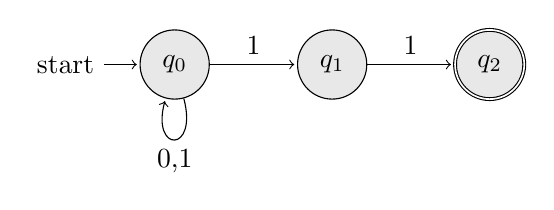
\begin{tikzpicture}[shorten >=1pt,node distance=2cm,auto]
  \tikzstyle{every state}=[fill={rgb:black,1;white,10}]

  \node[state,initial]   (q_0)                 {$q_0$};
  \node[state]           (q_1) [right of=q_0]  {$q_1$};
  \node[state,accepting] (q_2) [right of=q_1]  {$q_2$};

  \path[->]
  (q_0) edge                    node {1}        (q_1)
  (q_0) edge [loop below]       node {0,1}      ()
  (q_1) edge                    node {1}        (q_2)
  ;
\end{tikzpicture}

\begin{enumerate}
  \item The state $q_0$ has \textbf{more than one} possible transitions for the input $1$: it could go to state $q_1$,
        or it could go back to itself.
  \item The state $q_1$ has \textbf{zero} transition for the input $0$: the input $0$ makes no sense in the context of
        $q_1$. When we are in the state $q_1$ but then the input is $0$, we say the automaton \textbf{dies} and this
        particular series of choices do not accept.
\end{enumerate}

\colorbox{lime}{\textbf{NOTE(ywen)}}: Understanding ``any series of transitions'': Given the NFA above, consider the
input ``$1 \rightarrow 0 \rightarrow 1 \rightarrow 1$''. There are a few ways to go through the NFA:

\begin{enumerate}
  \item $q_0 \rightarrow q_0 \rightarrow q_0 \rightarrow q_0 \rightarrow q_0$: reject
  \item $q_0 \rightarrow q_0 \rightarrow q_0 \rightarrow q_0 \rightarrow q_1$: reject
  \item $q_0 \rightarrow q_0 \rightarrow q_0 \rightarrow q_1 \rightarrow q_2$: \textbf{accept}
  \item $q_0 \rightarrow q_1 $: die (i.e., reject)
\end{enumerate}

Each one is a series of transitions to go through the NFA. ``any series of transitions'' means if any one of the
possible series of transitions can lead to acceptance (i.e., the 3rd series in the example above), the input is
considered accepted.

% ******************************
\subsection{The \texorpdfstring{$\epsilon$}{}-Transitions}
% ******************************

The $\epsilon$-transitions are \textbf{NFA-specific}. An NFA may follow \textbf{any number} of $\epsilon$-transitions
at \textbf{any time} without consuming \textbf{any input}. NFAs are \textbf{not required} to follow $\epsilon$-
transitions. It's simply another option at the machine's disposal.

For example, given the following NFA,

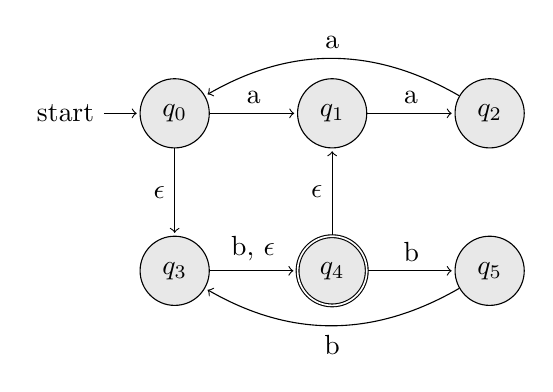
\begin{tikzpicture}[shorten >=1pt,node distance=2cm,auto]
  \tikzstyle{every state}=[fill={rgb:black,1;white,10}]

  \node[state,initial]   (q_0)                 {$q_0$};
  \node[state]           (q_1) [right of=q_0]  {$q_1$};
  \node[state]           (q_2) [right of=q_1]  {$q_2$};
  \node[state]           (q_3) [below of=q_0]  {$q_3$};
  \node[state,accepting] (q_4) [right of=q_3]  {$q_4$};
  \node[state]           (q_5) [right of=q_4]  {$q_5$};

  \path[->]
  (q_0) edge                    node {a}             (q_1)
  (q_0) edge [swap]             node {$\epsilon$}    (q_3)
  (q_1) edge                    node {a}             (q_2)
  (q_2) edge [bend right, swap] node {a}             (q_0)
  (q_3) edge                    node {b, $\epsilon$} (q_4)
  (q_4) edge                    node {$\epsilon$}    (q_1)
  (q_4) edge                    node {b}             (q_5)
  (q_5) edge [bend left]        node {b}             (q_3)
  ;
\end{tikzpicture}

consider the series of choices ``$b \rightarrow a \rightarrow a \rightarrow b \rightarrow b$''. There is no transition
on the input $b$ in the starting state $q_0$. However, because $q_0$ has an $\epsilon$-transition, before the first
input choice $b$ is consumed, the automaton can transition from $q_0$ to $q_3$ which has a transition on $b$. Likewise,
$q_4$ doesn't have any transition for $a$, but it has an $\epsilon$-transition to $q_1$ which has a transition on $a$.

The input series of choices ``$b \rightarrow a \rightarrow a \rightarrow b \rightarrow b$'' lead to the accepting state
by going through the states in the following sequence from $q_0$:

\[
  \epsilon \rightarrow b \rightarrow \epsilon \rightarrow a \rightarrow a \rightarrow \epsilon \rightarrow \epsilon
  \rightarrow b \rightarrow b \rightarrow \epsilon
\]

Note that the $\epsilon$-transitions were applied at the very beginning and at the very end. This is what ``\textbf{any
  time}'' means.

% ******************************
\subsection{NFA: Perfect positive guessing} \label{automata:nfa:perfect-positive-guessing}
% ******************************

Perfect positive guessing means an NFA has the \textbf{magical superpower} that enables them to guess choices that lead
to an accepting state. (If there are no such choices, the NFA guesses any one of the wrong guesses.)

For example, given the following NFA,

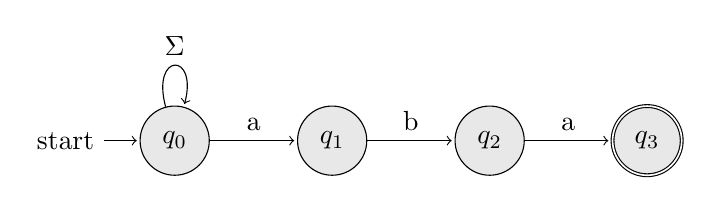
\begin{tikzpicture}[shorten >=1pt,node distance=2cm,auto]
  \tikzstyle{every state}=[fill={rgb:black,1;white,10}]

  \node[state,initial]   (q_0)                 {$q_0$};
  \node[state]           (q_1) [right of=q_0]  {$q_1$};
  \node[state]           (q_2) [right of=q_1]  {$q_2$};
  \node[state,accepting] (q_3) [right of=q_2]  {$q_3$};

  \path[->]
  (q_0) edge                    node {a}        (q_1)
  (q_0) edge [loop above]       node {$\Sigma$} ()
  (q_1) edge                    node {b}        (q_2)
  (q_2) edge                    node {a}        (q_3)
  ;
\end{tikzpicture}

consider the input ``$a \rightarrow b \rightarrow a \rightarrow b \rightarrow a$''. To land on the accepting state
$q_3$, the right transitions to go are $q_0 \rightarrow q_0 \rightarrow q_0 \rightarrow q_1 \rightarrow q_2 \rightarrow
  q_3$. The ``magical superpower'' means the NFA can magically figures out these transitions to choose them to arrive
at the accepting state.

This magical superpower has something to do with the property of NFAs that ``the machine \textbf{accepts} (the input)
if \textbf{any} series of transitions leads to an accepting state.'' See \ref{automata:nfa:definition-and-properties}.

However, as the course slides said:

\begin{displayquote}
  There is no known way to physically model this intuition of nondeterminism - this is quite a departure from reality!
\end{displayquote}

% ******************************
\subsection{NFA: Massive parallelism}
% ******************************

An NFA can be thought of as a DFA that can be \textbf{in many states at once}. At each point in time, when the NFA
needs to follow a transition, it tries \textbf{all the options at the same time}.

Use the same NFA as in the section \ref{automata:nfa:perfect-positive-guessing} for example. Consider the same series
of transitions ``$a \rightarrow b \rightarrow a \rightarrow b \rightarrow a$''. Initially, the NFA starts at $q_0$. For
the first transition ``a'', it can move to two states: going through the $\Sigma$ transition back to itself; going
through the $a$ transition to $q_1$. Massive parallelism says the NFA can do these two transitions at the same time,
ending up in both states (\colorbox{yellow}{yellow} and \colorbox{green}{green}):

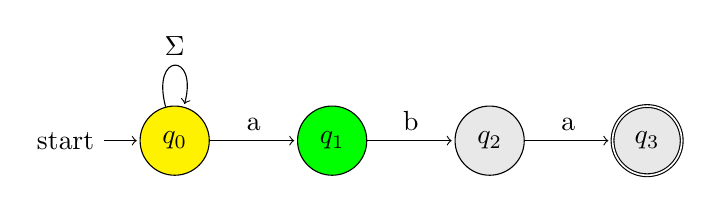
\begin{tikzpicture}[shorten >=1pt,node distance=2cm,auto]
  \tikzstyle{every state}=[fill={rgb:black,1;white,10}]

  \node[state,initial,fill=yellow]   (q_0)                 {$q_0$};
  \node[state,fill=green]            (q_1) [right of=q_0]  {$q_1$};
  \node[state]                       (q_2) [right of=q_1]  {$q_2$};
  \node[state,accepting]             (q_3) [right of=q_2]  {$q_3$};

  \path[->]
  (q_0) edge                    node {a}        (q_1)
  (q_0) edge [loop above]       node {$\Sigma$} ()
  (q_1) edge                    node {b}        (q_2)
  (q_2) edge                    node {a}        (q_3)
  ;
\end{tikzpicture}

The next transition is ``b''. Because now the NFA is at both $q_0$ and $q_1$, both of which can do the transition $b$,
so the NFA can do both again. $q_0$ still moves to itself; $q_1$ moves to $q_2$. See the following result.

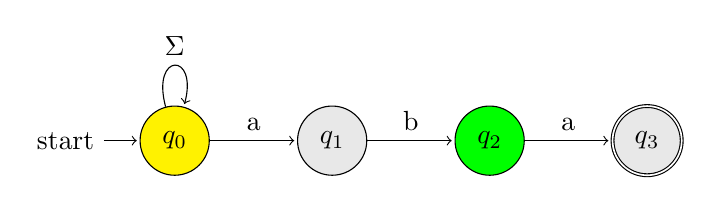
\begin{tikzpicture}[shorten >=1pt,node distance=2cm,auto]
  \tikzstyle{every state}=[fill={rgb:black,1;white,10}]

  \node[state,initial,fill=yellow]   (q_0)                 {$q_0$};
  \node[state]                       (q_1) [right of=q_0]  {$q_1$};
  \node[state,fill=green]            (q_2) [right of=q_1]  {$q_2$};
  \node[state,accepting]             (q_3) [right of=q_2]  {$q_3$};

  \path[->]
  (q_0) edge                    node {a}        (q_1)
  (q_0) edge [loop above]       node {$\Sigma$} ()
  (q_1) edge                    node {b}        (q_2)
  (q_2) edge                    node {a}        (q_3)
  ;
\end{tikzpicture}

The next transition is ``a'' again. Now there are three possible transitions to do: $q_0 \rightarrow q_0$,
$q_0 \rightarrow q_1$, $q_2 \rightarrow q_3$. Massive parallelism says they can all happen at the same time, resulting
in the new states below:

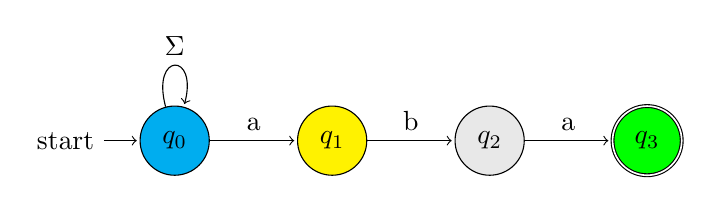
\begin{tikzpicture}[shorten >=1pt,node distance=2cm,auto]
  \tikzstyle{every state}=[fill={rgb:black,1;white,10}]

  \node[state,initial,fill=cyan]     (q_0)                 {$q_0$};
  \node[state,fill=yellow]           (q_1) [right of=q_0]  {$q_1$};
  \node[state]                       (q_2) [right of=q_1]  {$q_2$};
  \node[state,accepting,fill=green]  (q_3) [right of=q_2]  {$q_3$};

  \path[->]
  (q_0) edge                    node {a}        (q_1)
  (q_0) edge [loop above]       node {$\Sigma$} ()
  (q_1) edge                    node {b}        (q_2)
  (q_2) edge                    node {a}        (q_3)
  ;
\end{tikzpicture}

The next transition is ``b''. The state $q_3$ doesn't have a transition defined for ``b'', so we say the NFA
\textbf{dies} for this particular choice of transitions. But the transition ``b'' still works for $q_0$ and $q_1$. So
the NFA's new state will be as follows:

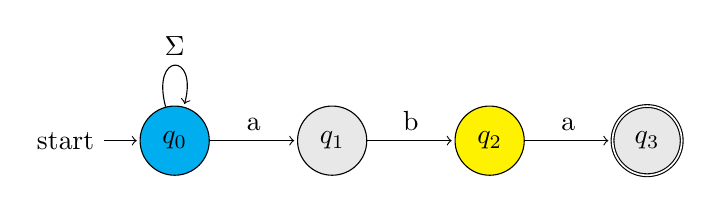
\begin{tikzpicture}[shorten >=1pt,node distance=2cm,auto]
  \tikzstyle{every state}=[fill={rgb:black,1;white,10}]

  \node[state,initial,fill=cyan]     (q_0)                 {$q_0$};
  \node[state]                       (q_1) [right of=q_0]  {$q_1$};
  \node[state,fill=yellow]           (q_2) [right of=q_1]  {$q_2$};
  \node[state,accepting]             (q_3) [right of=q_2]  {$q_3$};

  \path[->]
  (q_0) edge                    node {a}        (q_1)
  (q_0) edge [loop above]       node {$\Sigma$} ()
  (q_1) edge                    node {b}        (q_2)
  (q_2) edge                    node {a}        (q_3)
  ;
\end{tikzpicture}

The last transition is ``a''. At this moment, the NFA is at the state $q_0$ and $q_2$. Its previous state $q_3$ had
``died''. The new state will be as follows:

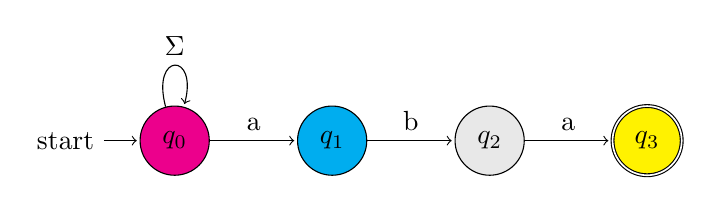
\begin{tikzpicture}[shorten >=1pt,node distance=2cm,auto]
  \tikzstyle{every state}=[fill={rgb:black,1;white,10}]

  \node[state,initial,fill=magenta]  (q_0)                 {$q_0$};
  \node[state,fill=cyan]             (q_1) [right of=q_0]  {$q_1$};
  \node[state]                       (q_2) [right of=q_1]  {$q_2$};
  \node[state,accepting,fill=yellow] (q_3) [right of=q_2]  {$q_3$};

  \path[->]
  (q_0) edge                    node {a}        (q_1)
  (q_0) edge [loop above]       node {$\Sigma$} ()
  (q_1) edge                    node {b}        (q_2)
  (q_2) edge                    node {a}        (q_3)
  ;
\end{tikzpicture}

Now we've finished running all the transitions. We are in at least one accepting state (the \colorbox{yellow}{$q_3$}),
so there is some path that gets us to an accepting state.

In contrast, the input sequence ``$a \rightarrow b \rightarrow a \rightarrow b$'' will not lead to any accepting state.
See the course slides for the detailed state changes.

% ******************************
\subsection{Designing NFAs}
% ******************************

A good model for designing NFAs: \textbf{guess-and-check}:
\begin{itemize}
  \item Is there some information that you'd really like to have? Have the machine \textbf{nondeterministically guess}
        that information.
  \item Then, have the machine \textbf{deterministically check} that the choice was correct.
\end{itemize}

\colorbox{lime}{\textbf{NOTE(ywen)}}: According to my own experience, given a problem:
\begin{itemize}
  \item It seems to be helpful to \textbf{directly} describe the \textbf{desired ending states}, and then figure out
        where the nondeterminism can fit in.
  \item Remember NFAs have two special devices:
        \begin{itemize}
          \item The $\epsilon$-transitions.
          \item An NFA can die to indicate the input is rejected.
        \end{itemize}
\end{itemize}

The course slides provide two examples. The second example demonstrates the use of the two devices: Design an automaton
that recognizes the language $L = \{ w \in \{a, b, c\}* | at \ least \ one \ of \ a, b, or \ c \ is \ not \ in \ w \}$.
The DFA solution is complicated (see the course slides), but the NFA solution is more simple:

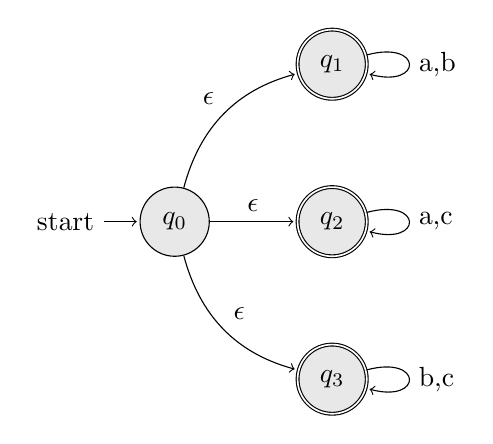
\begin{tikzpicture}[shorten >=1pt,node distance=2cm,auto]
  \tikzstyle{every state}=[fill={rgb:black,1;white,10}]

  \node[state,initial]     (q_0)                 {$q_0$};
  \node[state,accepting]   (q_2) [right of=q_0]  {$q_2$};
  \node[state,accepting]   (q_1) [above of=q_2]  {$q_1$};
  \node[state,accepting]   (q_3) [below of=q_2]  {$q_3$};

  \path[->]
  (q_0) edge [bend left]  node {$\epsilon$}      (q_1)
  (q_1) edge [loop right] node {a,b}             ()
  (q_0) edge              node {$\epsilon$}      (q_2)
  (q_2) edge [loop right] node {a,c}             ()
  (q_0) edge [bend right] node {$\epsilon$}      (q_3)
  (q_3) edge [loop right] node {b,c}             ()
  ;
\end{tikzpicture}

If the input sequence doesn't contain ``a'', the solution relies on the NFA be able to magically pick the
$\epsilon$-transition to $q_3$; if the input sequence doesn't contain ``b'', the solution relies on the NFA be able to
magically pick the $\epsilon$-transition to $q_2$; if the input sequence doesn't contain ``c'', the solution relies on
the NFA be able to magically pick the $\epsilon$-transition to $q_1$.

If the input sequence contains all the letters ``a'', ``b'', and ``c'', it doesn't matter which transition to take at
$q_0$. The NFA will always die at a point, which indicates the rejection of the input.

% =============================================================================
\section{Describe DFAs and NFAs as tables}
% =============================================================================

DFAs and NFAs are essentially graphs, so we can use adjacent matrices (with some modifications) to describe them.

% ******************************
\subsection{Tabular DFAs}
% ******************************

Because a DFA is deterministic, the state of the DFA after a transition can be completely described by a state in the
DFA, so the transitions are truly from one state to another state.

For example, given the following DFA:

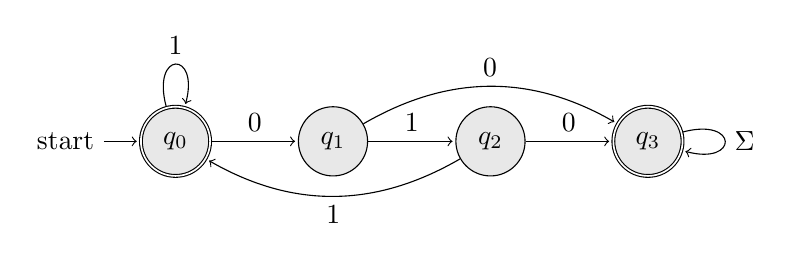
\begin{tikzpicture}[shorten >=1pt,node distance=2cm,auto]
  \tikzstyle{every state}=[fill={rgb:black,1;white,10}]

  \node[state,initial,accepting] (q_0) {$q_0$};
  \node[state]                   (q_1) [right of=q_0] {$q_1$};
  \node[state]                   (q_2) [right of=q_1]{$q_2$};
  \node[state,accepting]         (q_3) [right of=q_2] {$q_3$};

  \path[->]
  (q_0) edge [loop above] node {1}        ()
  (q_0) edge              node {0}        (q_1)
  (q_1) edge              node {1}        (q_2)
  (q_1) edge [bend left]  node {0}        (q_3)
  (q_2) edge              node {0}        (q_3)
  (q_2) edge [bend left]  node {1}        (q_0)
  (q_3) edge [loop right] node {$\Sigma$} (q_3)
  ;
\end{tikzpicture}

We can use the following modified adjacent matrix to describe it with two modifications:
\begin{enumerate}
  \item The first row is the starting state.
  \item The asterisks (``*'') indicate the accepting states.
\end{enumerate}

\begin{table}[H]
  \begin{tabular}{|c|c|c|ll}
    \cline{1-3}
           & 0     & 1     &  & \\ [1ex]   \cline{1-3}
    *$q_0$ & $q_1$ & $q_0$ &  & \\ [0.5ex] \cline{1-3}
    $q_1$  & $q_3$ & $q_2$ &  & \\ [0.5ex] \cline{1-3}
    $q_2$  & $q_3$ & $q_0$ &  & \\ [0.5ex] \cline{1-3}
    *$q_3$ & $q_3$ & $q_3$ &  & \\ [0.5ex] \cline{1-3}
  \end{tabular}
\end{table}

% ******************************
\subsection{Tabular NFAs} \label{automata:tabular-nfas}
% ******************************

Because an NFA is nondeterministic, the state of the NFA after a transition are described by a set of states in the NFA
due to the massive parallelism, so the transitions are actually from one set of states to another set of states.

For example, given the following NFA:

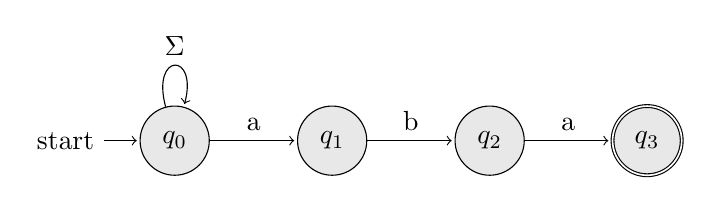
\begin{tikzpicture}[shorten >=1pt,node distance=2cm,auto]
  \tikzstyle{every state}=[fill={rgb:black,1;white,10}]

  \node[state,initial]   (q_0)                {$q_0$};
  \node[state]           (q_1) [right of=q_0] {$q_1$};
  \node[state]           (q_2) [right of=q_1] {$q_2$};
  \node[state,accepting] (q_3) [right of=q_2] {$q_3$};

  \path[->]
  (q_0) edge [loop above] node {$\Sigma$} ()
  (q_0) edge              node {a}        (q_1)
  (q_1) edge              node {b}        (q_2)
  (q_2) edge              node {a}        (q_3)
  ;
\end{tikzpicture}

We can use the following adjacent matrix to describe it:

\begin{table}[H]
  \begin{tabular}{|c|c|c|ll}
    \cline{1-3}
                         & a                   & b              &  & \\ [1ex]   \cline{1-3}
    \{$q_0$\}            & \{$q_0, q_1$\}      & \{$q_0$\}      &  & \\ [0.5ex] \cline{1-3}
    \{$q_0, q_1$\}       & \{$q_0, q_1$\}      & \{$q_0, q_2$\} &  & \\ [0.5ex] \cline{1-3}
    \{$q_0, q_2$\}       & \{$q_0, q_1, q_3$\} & \{$q_0$\}      &  & \\ [0.5ex] \cline{1-3}
    *\{$q_0, q_1, q_3$\} & \{$q_0, q_1$\}      & \{$q_0, q_2$\} &  & \\ [0.5ex] \cline{1-3}
  \end{tabular}
\end{table}

This can be viewed as a DFA as follows:

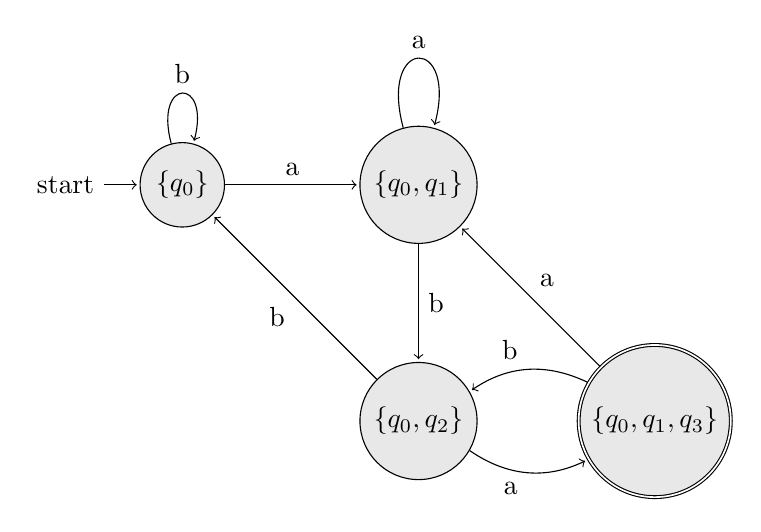
\begin{tikzpicture}[shorten >=1pt,node distance=3cm,auto]
  \tikzstyle{every state}=[fill={rgb:black,1;white,10}]

  \node[state,initial]   (q0) {\{$q_0$\}};
  \node[state]           (q0q1) [right of=q0] {\{$q_0, q_1$\}};
  \node[state]           (q0q2) [below of=q0q1]{\{$q_0, q_2$\}};
  \node[state,accepting] (q0q1q3) [right of=q0q2] {\{$q_0, q_1, q_3$\}};

  \path[->]
  (q0) edge [loop above]           node {b} ()
  (q0) edge                        node {a} (q0q1)
  (q0q1) edge [loop above]         node {a} ()
  (q0q1) edge                      node {b} (q0q2)
  (q0q2) edge [bend right, swap]   node {a} (q0q1q3)
  (q0q2) edge                      node {b} (q0)
  (q0q1q3) edge [bend right, swap] node {b} (q0q2)
  (q0q1q3) edge [swap]             node {a} (q0q1)
  ;
\end{tikzpicture}

% =============================================================================
\section{The Regular Languages}
% =============================================================================

% ******************************
\subsection{Definition}
% ******************************

A language $L$ is called a \textbf{regular language} if there exists a DFA $D$ such that $\mathfrak{L}(D) = L$.
If $L$ is a language and $\mathfrak{L}(D) = L$, we say that $D$ \textbf{recognizes} the language $L$.

\colorbox{lime}{\textbf{NOTE(ywen)}}: The section \ref{automata:automata-and-languages} talks about the languages from
the perspective of a DFA: given a DFA, the strings that this DFA accepts form the language of this DFA. Here, we are
talking about the languages from the perspective of the language itself: given a language, how can we tell if it is
regular or not? It depends on whether there exists a DFA to define this language.

% ******************************
\subsection{NFA's language and DFA's language}
% ******************************

Remember that the language of an automaton is the set of the inputs that the automaton accepts. Therefore, the language
of the NFA in \ref{automata:tabular-nfas} is the same as the language of the DFA which was converted from the NFA.

\textbf{Theorem}: A language $L$ is regular $\Leftrightarrow$ $\exists N: \mathfrak{L}(N) = L$. (See the course slides
for a sketchy proof.)

% ******************************
\subsection{Properties}
% ******************************

Given a language $L \subseteq \Sigma*$, the \textbf{complement} of that language (denoted $\bar{L}$) is the language of
all strings in $\Sigma*$ that aren't in $L$. Formally: $L = \Sigma* - L$.

If $L$ is a regular language, that means there exists a DFA $D$ that recognizes $L$. We can construct the DFA of $L$'s
complement by changing all the accepting states in $D$ to non-accepting states, and changing all the non-accepting
states in $D$ to accepting states. For example:

L = \{ w $\in$ \{a, b\}* $|$ w contains ``aa'' as a substring \}

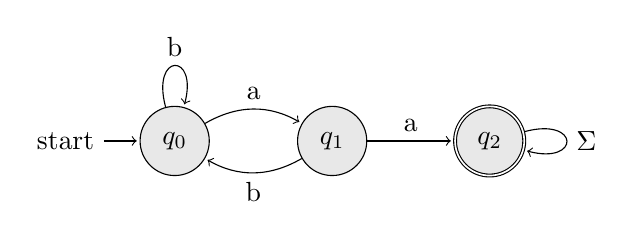
\begin{tikzpicture}[shorten >=1pt,node distance=2cm,auto]
  \tikzstyle{every state}=[fill={rgb:black,1;white,10}]

  \node[state,initial]   (q_0)                {$q_0$};
  \node[state]           (q_1) [right of=q_0] {$q_1$};
  \node[state,accepting] (q_2) [right of=q_1] {$q_2$};

  \path[->]
  (q_0) edge [loop above] node {b} ()
  (q_0) edge [bend left]  node {a}        (q_1)
  (q_1) edge              node {a}        (q_2)
  (q_1) edge [bend left]  node {b}        (q_0)
  (q_2) edge [loop right] node {$\Sigma$} (q_3)
  ;
\end{tikzpicture}

$\bar{L}$ = \{ w $\in$ \{a, b\}* $|$ w \textbf{does not} contain ``aa'' as a substring \}

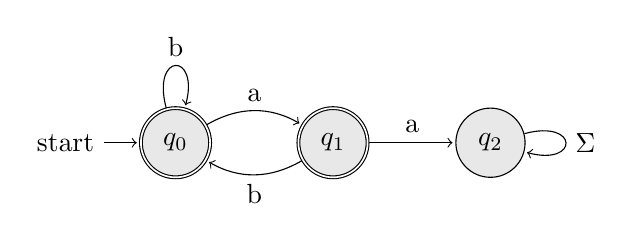
\begin{tikzpicture}[shorten >=1pt,node distance=2cm,auto]
  \tikzstyle{every state}=[fill={rgb:black,1;white,10}]

  \node[state,initial,accepting] (q_0)                {$q_0$};
  \node[state,accepting]         (q_1) [right of=q_0] {$q_1$};
  \node[state]                   (q_2) [right of=q_1] {$q_2$};

  \path[->]
  (q_0) edge [loop above] node {b} ()
  (q_0) edge [bend left]  node {a}        (q_1)
  (q_1) edge              node {a}        (q_2)
  (q_1) edge [bend left]  node {b}        (q_0)
  (q_2) edge [loop right] node {$\Sigma$} (q_3)
  ;
\end{tikzpicture}

Therefore: If $L$ is a regular language, then $\bar{L}$ is also a regular language. As a result, we say that the
regular languages are \textbf{closed under complementation}.

We also have: If $L_1$ and $L_2$ are regular languages, then:
\begin{enumerate}
  \item $L_1 \cup L_2$ is regular. (The proof uses $\epsilon$-transitions of NFAs.)
  \item $L_1 \cap L_2$ is regular. (The proof uses De Morgan laws.)
\end{enumerate}

% =============================================================================
%
% Regular Expression
%
% =============================================================================

\chapter{Regular Expression}

 (TODO)

% =============================================================================
%
% Nonregular Languages
%
% =============================================================================

\chapter{Nonregular Languages}

 (TODO)

% =============================================================================
%
% Context-Free Languages
%
% =============================================================================

\chapter{Context-Free Languages}

 (TODO)

% =============================================================================
%
% Turing Machines
%
% =============================================================================

\chapter{Turing Machines}

 (TODO)

% =============================================================================
%
% Unsolvable Problems
%
% =============================================================================

\chapter{Unsolvable Problems}

 (TODO)

% =============================================================================
%
% Complexity Theory and P vs NP
%
% =============================================================================

\chapter{Complexity Theory and P vs NP}

 (TODO)

\chapter*{References}
\addcontentsline{toc}{chapter}{References}

\begin{itemize}
  \item $[1]$ \href{https://web.stanford.edu/class/cs103/}{CS103: Mathematical Foundations of Computing}
\end{itemize}

\end{document}
